\documentclass[a4paper, 12pt]{book}

\usepackage{times}
\usepackage{verbatim}
\usepackage{color}
\usepackage{url}
\usepackage{graphicx}
\usepackage{array}

% uncomment this if you want to indent the first paragraph
%\usepackage{indentfirst}

% uncomment this if you want to make pdf file with hyperlink
% \usepackage[dvipdf,colorlinks=false,unicode]{hyperref}

% uncomment the following and correct them if you want to set 
% set the pdf properties
%\hypersetup{
%	pdfauthor={Tz-Huan Huang},
%	pdftitle={A Benchmark for Region-of-Interest Detection in Images},
%	pdfsubject={Master Thesis}
%}

\usepackage{ntu}

%\usepackage{xeCJK}
%\setCJKmainfont{標楷體}

\setcounter{tocdepth}{2}

\pagestyle{plain}

\begin{document}

% cover page
\maketitle

% side page, used for printing on spline.
\makeside

\frontmatter

%\begin{CJK}{Bg5}{cwku}
\begin{CJK}{UTF8}{zhkai}
\CJKhorz
%\makecertification

% comment one of the following unless you are sure you want to 
% have both english and chinese acknowledgements in your thesis
\begin{acknowledgementsEN}

I'm glad to thank \ldots

\end{acknowledgementsEN}

\begin{acknowledgementsCH}

\setlength{\baselineskip}{1.5em}
感謝\ldots

\end{acknowledgementsCH}


\begin{abstractCH}

\setlength{\baselineskip}{1.5em}
本論文提出了一影像中使用者感興趣區域 (region of interest) 偵測%
之資料集 (benchmark)。%
使用者感興趣區域偵測在許多應用中極為有用,%
過去雖然有許多使用者感興趣區域之自動偵測演算法被提出,%
然而由於缺乏公開資料集,%
這些方法往往只測試了各自的小量資料而難以互相比較。%
從其它領域可以發現,%
基於公開資料集的可重製實驗與該領域突飛猛進密切相關,
因此本論文填補了此領域之不足,%
我們提出名為「Photoshoot」的遊戲來蒐集人們對於感興趣區域的標記,%
並以這些標記來建立資料集。%
透過這個遊戲,我們已蒐集大量使用者對於感興趣區域的標記,%
並結合這些資料成為使用者感興趣區域模型。%
我們利用這些模型來量化評估五個使用者感興趣區域偵測演算法,%
此資料集也可更進一步作為基於學習理論演算法的測試資料,%
因此使基於學習理論的偵測演算法成為可能。

\end{abstractCH}

\begin{abstractEN}

This thesis presents a benchmark for region of interest (ROI)
detection. ROI detection has many useful applications and many
algorithms have been proposed to automatically detect ROIs.
Unfortunately, due to the lack of benchmarks, these methods were
often tested on small data sets that are not available to others,
making fair comparisons of these methods difficult. Examples from
many fields have shown that repeatable experiments using published
benchmarks are crucial to the fast advancement of the fields. To
fill the gap, this thesis presents our design for a collaborative
game, called Photoshoot, to collect human ROI annotations for
constructing an ROI benchmark. With this game, we have gathered a
large number of annotations and fused them into aggregated ROI
models. We use these models to evaluate five ROI detection
algorithms quantitatively. Furthermore, by using the benchmark as
training data, learning-based ROI detection algorithms become
viable.

\end{abstractEN}

\begin{comment}

\category{I2.10}{Computing Methodologies}{Artificial Intelligence --
Vision and Scene Understanding} \category{H5.3}{Information
Systems}{Information Interfaces and Presentation (HCI) -- Web-based
Interaction.}

\terms{Design, Human factors, Performance.}

\keywords{Region of interest, Visual attention model, Web-based
games, Benchmarks.}

\end{comment}

\tableofcontents
\end{CJK}
\listoffigures
\listoftables

\mainmatter

% input your thesis here
\chapter{Introduction}
\label{c:intro}

% Background, Motivation and Relevant work
Attention plays an important role in human vision. For example, when
we look at an image, our eye movements comprise a succession of {\em
fixations} (repetitive positioning of eyes to parts of the image)
and {\em saccades} (rapid eye jump). Those parts of the image that
cause eye fixations and capture primary attention are called {\em
regions of interest} (ROIs). Studies in visual attention and eye
movement have shown that humans generally only attend to a few ROIs.
Detecting these visually attentive regions in images is challenging
but useful in many multimedia applications, such as automatic
thumbnail cropping, object recognition, content-based image
retrieval, adaptive image compression and automatic browsing in
small-screen devices.

Describe the common dilemma between exploration and exploitation for real-valued optimization algorithms.
Describe our basic assumption that problems worth solving are hierarchical decomposable~\cite{herbsimon:}.

% Thesis Objective
\section{Thesis Objectives}
We propose a technique that helps identify {\em regions of interest} (ROI) to explore and \textit{allocate resources} according to remaining evaluations.

First, describe why is it important to identify ROIs.
Describe how subspace projection creates a \textit{well-defined boundary} that some algorithms need.
Describe how subspace projection helps  solve \textit{inseparable problems} while enhance the ability to find optimium.

Second, describe how the proposed resources allocation benefits optimization.
Describe different strategies one should take given different evaluations left.
Describe how Multi-armed Bandit (MAB) algorithms are suitable for the scenario, instead of decision theory, reinforcement learning and Markov Decision Process.
MAB learns models from outcomes while the actions do not change the state of the world.


\section{Roadmap}
This thesis is composed of seven chapters.


\textbf{Chapter~\ref{chapter:algos}} presents three optimization algorithms that are adopted for comparisons. 
These three algorithms each have different characteristics. 
The Covariance Matrix Adaptation Evolutionary Strategy.
The Standard Particle Swarm Optimization.
The Ant Colony Optimization for Continous Domain.


\textbf{Chapter~\ref{chapter:clustering}} presents some clustering techniques that guides the construction of ROIs and later becomes the initial points for algorithms in each arm.


\textbf{Chapter~\ref{chapter:projection}} first describes four basic affine transformation: translation, rotation, scaling and shearing.
Then the projective transformation and homogeneous coordinate are presented.


\textbf{Chapter~\ref{chapter:MAB}} briefly describes some common multi-armed bandit algorithms, including ...
Then we present our new bandit techniques.
Tranditional bandit algorithms focus on minimizing regret, while our new bandit focus on the probability of getting a rank 1 result.


\textbf{Chapter~\ref{chapter:new_bandit}} gives details of our new algorithms.
First, the framework and pseudo code are given.
Then a detailed process of initialization is given in ...
% talk about ROI, what it is, why it is important

\textbf{Chapter~\ref{chapter:conclusion}} summarizes this thesis. 
The conclusion and contributions are also given.
Some further improvements and future works are also discussed at the end.



\chapter{Real-valued Optimization Algorithms}
\label{chapter:algos}

Overview of real-valued optimization

\section{Covariance Matrix Adaptation Evolution Strategy}

Describe history of \textit{Evolutionary Strategies} (ES).
The simplest algorithm is (1+1)-ES.
Here we describe the (1+1)-ES with one-fifth success rule with independent restarts.
The pseudo code of (1+1)-ES is given in Algorithm~\ref{algo:1+1ES}.

Covariance Matrix Adaptation Evolution Strategy (CMA-ES) is an extended version fo CSA-ES with de-randomized adaptation of covariance matrix.
Describe the underlying covariance matrix model.

Describe how to update \textit{mean}.

Describe how to update \textit{covariance matrix}.

Describe \textit{step-size} control.



\begin{algorithm}%[t!]
\caption{(1+1)-ES with 1/5 success-rule}\label{algo:1+1ES}

$\boldsymbol{X}_{n}$: solution of the $n^{th}$ iteration, $\sigma_n$: step size of the $n^{th}$ iteration, \\
$N(\boldsymbol{0}, \boldsymbol{I})$: multivariant normal distribution with mean vector $\boldsymbol{0}$ \\ 
and identical covariance matrix $\boldsymbol{I}$.

\BlankLine
\SetKwInOut{Input}{input} \SetKwInOut{Output}{output}
\Input{ $f$: evaluation function }
\Output{ $X_{n+1}$: best solution }

\BlankLine
Initialize $\boldsymbol{X}_0, \sigma_0$ \\
\While{ termination criterion not met } {

    $\widetilde{\boldsymbol{X}}_n = \boldsymbol{X}_n + \sigma_n N(\boldsymbol{0}, \boldsymbol{I})$  \\

    \eIf{ $f(\widetilde{\boldsymbol{X}}_n) \leq f(\boldsymbol{X}_n) $}{
        $\boldsymbol{X}_{n+1} = \widetilde{\boldsymbol{X}}_n$ \\
        $\sigma_{n+1} = 1.5 \sigma_n$
    }{
        $\boldsymbol{X}_{n+1} = \boldsymbol{X}_n$ \\
        $\sigma_{n+1} = 1.5^{-1/4}\sigma_n$
    }
}

\Return $\boldsymbol{X}_{n+1}$

\end{algorithm}





\section{Standard Particle Swarm Optimization}

Particle Swarm Optimization was first proposed by ...
The swarm intelligence family... 
However, there are multiple varients of PSO over the years.

Standard PSO provides a well defined version of PSO that follows the basic principles.
It is intend to be a milestone for future comparison, instead of the best algorithm on the market.

So far, there have been three successive versions of standard PSO: SPSO 2006, 2007 and 2011
The underlying principles of these three versions are generally the same as all PSO varients.
The exact formula and implementation are slightly different due to latest theoretical progress.

Describe swarm size definition and basic elements for each particle.
Initialization of the swarm.
The swarm size, denoted as $S$, differs in SPSO 2006 and SPSO 2011.
In both SPSO 2006 and SPSO 2007, the initial number of particles for dimension $D$ is defined as:
\begin{displaymath}
S = 10 + \lfloor 2\sqrt{D} \rfloor,
\end{displaymath}
However, in SPSO 2011, the swarm size can be defined by user, yet suggested as 40~\cite{Clerc:2012:SPSO2011} since the original swarm size is far from optimal.

Each particle in the swarm possesses the following elements: current position, current velocity, personal pervious best position, and previous best position in the neighbourhood. 


Describe random topology and when to update topology.
The information links...
The adaptive random topology described in ~\cite{Clerc:2007:randomTopology} is formally equivalent to "Stocastic Star".

Describe velocity update for SPSO 2006 and SPSO 2011
Update Velocity as shown in Figure~\ref{fig:SPSO_update}
\begin{figure}
\centering
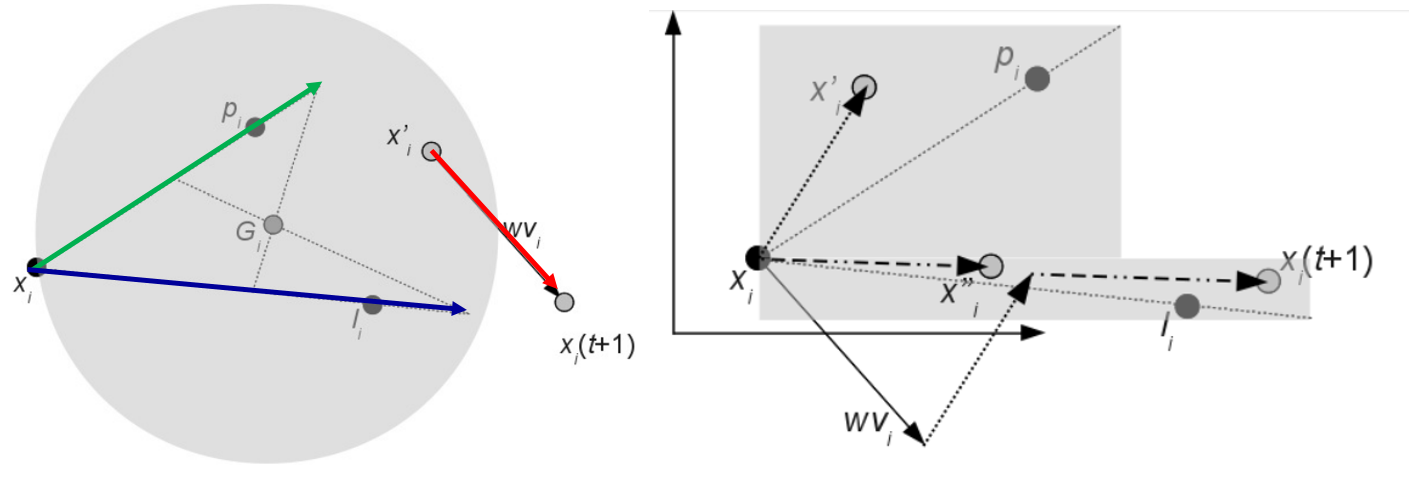
\includegraphics[width=\textwidth]{SPSO_update}
\caption{(a) SPSO 2011. (b) SPSO 2006.}\label{fig:SPSO_update}
\end{figure}

Describe boundary and out-of-bound handling.



The pseudo code defined in~\cite{Zambrano:2013:SPSO2011}.
The pseudo code is given in Algorithm~\ref{algo:SPSO2011}.



\begin{algorithm}%[t!]
\caption{Standard PSO 2011}\label{algo:SPSO2011}

$\boldsymbol{X}_{n}$: solution of the $n^{th}$ iteration, $\sigma_n$: step size of the $n^{th}$ iteration, \\
$N(\boldsymbol{0}, \boldsymbol{I})$: multivariant normal distribution with mean vector $\boldsymbol{0}$ \\ 
and identical covariance matrix $\boldsymbol{I}$.

\BlankLine
\SetKwInOut{Input}{input} \SetKwInOut{Output}{output}
\Input{ $f$: evaluation function }
\Output{ $X_{n+1}$: best solution }

\BlankLine
Initialize $\boldsymbol{X}_0, \sigma_0$ \\
\While{ termination criterion not met } {

    $\widetilde{\boldsymbol{X}}_n = \boldsymbol{X}_n + \sigma_n N(\boldsymbol{0}, \boldsymbol{I})$  \\

    \eIf{ $f(\widetilde{\boldsymbol{X}}_n) \leq f(\boldsymbol{X}_n) $}{
        $\boldsymbol{X}_{n+1} = \widetilde{\boldsymbol{X}}_n$ \\
        $\sigma_{n+1} = 1.5 \sigma_n$
    }{
        $\boldsymbol{X}_{n+1} = \boldsymbol{X}_n$ \\
        $\sigma_{n+1} = 1.5^{-1/4}\sigma_n$
    }
}

\Return $\boldsymbol{X}_{n+1}$

\end{algorithm}




\section{Ant Colony Optimization for Continuous Domain}

Ant Colony optimization (ACO) is first proposed by Dorigo~\cite{Dorigo:1999:ACO} to solve combinatorial optimization problems, including scheduling, routing, and timetabling.
These problems aim to find optimal \textit{combinations} or \textit{permutations} of finit sets of available components.
Inspired by the foraging behavior of natural ants, ACO mimics the pheromone deposition of ants along the trail to a food source.
The deposited pheromone, which indicates the quantity and quality of the food, creates an indirect communication among ants and enables them to find the shortest paths.
The pseudo code of ACO is given in Algorithm~\ref{algo:ACO}.
Two major procedures: \textit{solution construction} and \textit{phermone update}, are detailed in the following paragraph.


Consider a search space $\boldsymbol{S}$ defined over a finit set of all possible \textit{solution components}, denoted by $\boldsymbol{C}$.
Each solution component, denoted by $c_{ij}$, is a decision variable $X_i$ instantiated with value $v^{j}_{i} \in \boldsymbol{D}_i = \{ v^{1}_{i}, ..., v^{|\boldsymbol{D}_i|}_{i}\}$.
To construct a new solution, an artificial ants starts with an empty partial solution $s^{p} = \emptyset$.
During each construction step, the partial solution $s^{p}$ is extended with a feasible solution from the set $N(s^{p}) \in \boldsymbol{C} \setminus s^{p}$.
The probabilistic pheromone model adopted for selecting a feasible solution from $N(s^{p})$ can be defined as follows:

\begin{equation}
p(c_{ij}|s^p) = \frac{\tau^{\alpha}_{ij} \cdot \eta(c_{ij})^{\beta}} 
                     {\sum_{c_{i\ell}\in N(s^{p})} \tau^{\alpha}_{i\ell} \cdot \eta(c_{i\ell})^{\beta} },  \forall c_{ij} \in N(s^{p}),
\end{equation}
where $\tau_{ij}$ is the pheromone value associated with component $c_{ij}$, and $\eta(\cdot)$ is a weighting function. 
% that assigns at each construction step a heuristic value to each feasible solution component $c_{ij} \in N(s^{p})$.
$\alpha$ and $\beta$ are positive parameters which determine the relation between phermone and heuristic information.

The pheromone update


Over the years, multiple approaches of extending the ACO on continous domain have been given.
One of the most successful version is ACO$_{R}$, proposed by Socha and Dorigo in 2008~\cite{Socha:2008:ACOR}.
It extends ACO to the continuous domain without making any major conceptual change to its structure.
The fundamental idea underlying ACO$_{R}$ is the shift from using a discrete probability distribution to using a continuous one, demonstrated in Figure~\ref{fig:ACOR_distribution}. 

A enhanced Gaussian kernel PDF as shown in Figure~\ref{fig:ACOR_gaussianKernel}.

\begin{figure}
\centering
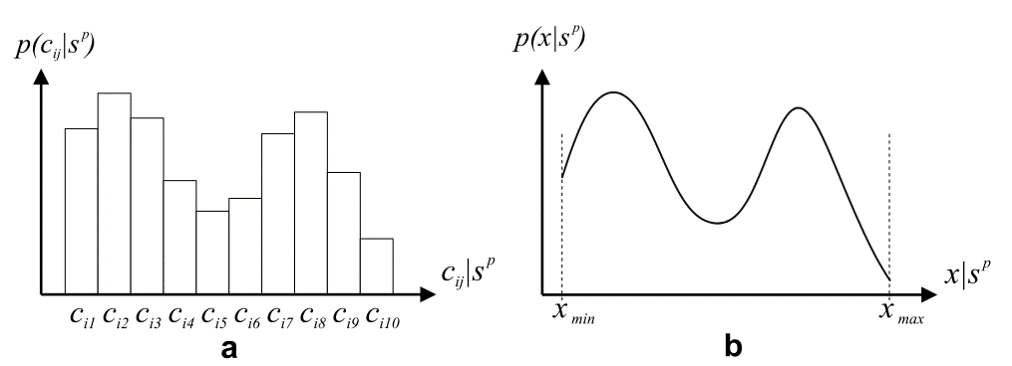
\includegraphics[width=\textwidth]{ACOR_distribution}
\caption{(a) Discrete probability distribution $p(c_{ij}|s^{p})$. (b) Continuous probability density function $p(x|s^{p})$}\label{fig:ACOR_distribution}
\end{figure}

\begin{figure}
\centering
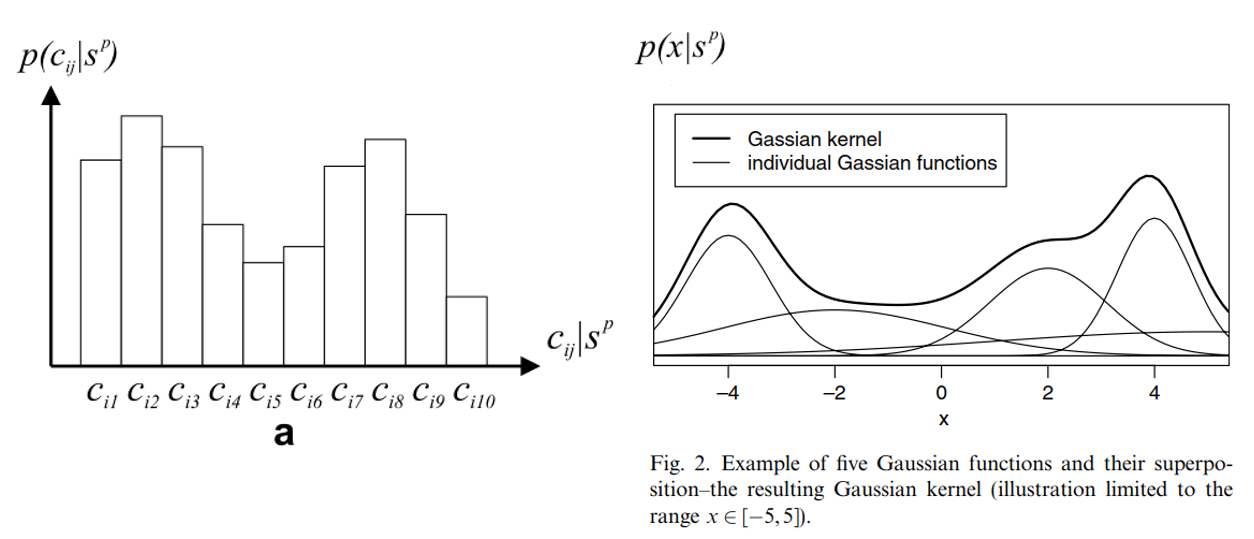
\includegraphics[width=\textwidth]{ACOR_gaussianKernel}
\caption{(a) Discrete probability distribution $p(c_{ij}|s^{p})$. (b) Continuous probability density function $p(x|s^{p})$}\label{fig:ACOR_gaussianKernel}
\end{figure}

\begin{algorithm}%[t!]
\caption{Ant Colony Optimization metaheuristic}\label{algo:ACO}
\While{ termination criterion not met } {

    schedule activities \\
    solution contruction by ants(); \\
    phermone update(); \\
    daemon actions(); \\
}
\end{algorithm}




\chapter{Multi-armed Bandit Algorithms}
\label{c:bandit}

% talk about ROI, what it is, why it is important
Describe the exploration vs. exploitation dilemma.

\section{The Multi-armed Bandit Problem}


\section{The Upper Confidence Bound Algorithm}


\section{The Price of Knowledge and Estimated Reward strategy}
The Price of Knowledge and Estimated Reward (POKER) strategy considers three ideas: pricing uncertainty, exploiting the lever distribution and taking into account the horizon


Attention plays an important role in human vision. For example, when
we look at an image, our eye movements comprise a succession of {\em
fixations} (repetitive positioning of eyes to parts of the image)
and {\em saccades} (rapid eye jump). Those parts of the image that
cause eye fixations and capture primary attention are called {\em
regions of interest} (ROIs). Studies in visual attention and eye
movement have shown that humans generally only attend to a few ROIs.
Detecting these visually attentive regions in images is challenging
but useful in many multimedia applications, such as automatic
thumbnail cropping, object recognition, content-based image
retrieval, adaptive image compression and automatic browsing in
small-screen devices.


\chapter{Linear Transformation}
\label{c:transformation}

% talk about ROI, what it is, why it is important
Overview of real-valued optimization

\section{Affine Transformation}

\subsection{Translation}
\subsection{Rotation}
\subsection{Scaling}
\subsection{Shear}
\subsection{Affine transformation matrix}
Augmented Matrix

\section{Projective Transformation}


\section{Optimization for Transformation Matrix}

Attention plays an important role in human vision. For example, when
we look at an image, our eye movements comprise a succession of {\em
fixations} (repetitive positioning of eyes to parts of the image)
and {\em saccades} (rapid eye jump). Those parts of the image that
cause eye fixations and capture primary attention are called {\em
regions of interest} (ROIs). Studies in visual attention and eye
movement have shown that humans generally only attend to a few ROIs.
Detecting these visually attentive regions in images is challenging
but useful in many multimedia applications, such as automatic
thumbnail cropping, object recognition, content-based image
retrieval, adaptive image compression and automatic browsing in
small-screen devices.


\chapter{The New Bandit Technique}
\label{c:new_bandit}

% talk about ROI, what it is, why it is important
Overview of real-valued optimization

\section{Framework of the New Bandit Algorithm}
\section{Initialize Clusters}
\section{Subspace Projection}
\section{Remain Evaluations Allocation}
\section{Recluster}



Attention plays an important role in human vision. For example, when
we look at an image, our eye movements comprise a succession of {\em
fixations} (repetitive positioning of eyes to parts of the image)
and {\em saccades} (rapid eye jump). Those parts of the image that
cause eye fixations and capture primary attention are called {\em
regions of interest} (ROIs). Studies in visual attention and eye
movement have shown that humans generally only attend to a few ROIs.
Detecting these visually attentive regions in images is challenging
but useful in many multimedia applications, such as automatic
thumbnail cropping, object recognition, content-based image
retrieval, adaptive image compression and automatic browsing in
small-screen devices.


\chapter{Experiments}
\label{c:experiments}

% talk about ROI, what it is, why it is important
Overview of real-valued optimization

\section{Test Problems}

\subsection{CEC2005 25 benchmark problems}

\section{Experiment Settings}

CMA-ES initial mean and std, population settings
SPSO2011 parameters (c, w) settings, and population settings

\section{Results}
\section{Discussion}



Attention plays an important role in human vision. For example, when
we look at an image, our eye movements comprise a succession of {\em
fixations} (repetitive positioning of eyes to parts of the image)
and {\em saccades} (rapid eye jump). Those parts of the image that
cause eye fixations and capture primary attention are called {\em
regions of interest} (ROIs). Studies in visual attention and eye
movement have shown that humans generally only attend to a few ROIs.
Detecting these visually attentive regions in images is challenging
but useful in many multimedia applications, such as automatic
thumbnail cropping, object recognition, content-based image
retrieval, adaptive image compression and automatic browsing in
small-screen devices.


\chapter{Conclusion}
\label{chapter:conclusion}


%\section{Test Problems}
Contribution:
find potential region to search
allocate resources

Weakness:
Potentially more NFE on unimodals and moving regions.
Requires a better clustering techniques to identify underlying unimodals.


Future work:
Non-linear transformation



Attention plays an important role in human vision. For example, when
we look at an image, our eye movements comprise a succession of {\em
fixations} (repetitive positioning of eyes to parts of the image)
and {\em saccades} (rapid eye jump). Those parts of the image that
cause eye fixations and capture primary attention are called {\em
regions of interest} (ROIs). Studies in visual attention and eye
movement have shown that humans generally only attend to a few ROIs.
Detecting these visually attentive regions in images is challenging
but useful in many multimedia applications, such as automatic
thumbnail cropping, object recognition, content-based image
retrieval, adaptive image compression and automatic browsing in
small-screen devices.



\backmatter

\addcontentsline{toc}{chapter}{\bibname}
\bibliographystyle{abbrv}

% input your reference here
% \bibliography{thesis}

\appendix

\end{document}
